

%% This file was auto-generated by IPython.
%% Conversion from the original notebook file:
%%
\documentclass[11pt,english]{article}

%% This is the automatic preamble used by IPython.  Note that it does *not*
%% include a documentclass declaration, that is added at runtime to the overall
%% document.

\usepackage{amsmath}
\usepackage{amssymb}
\usepackage{graphicx}
\usepackage{ucs}
\usepackage[utf8x]{inputenc}
\usepackage{caption}
\usepackage{subcaption}

\graphicspath{{debacl_tutorial_files/}}

% needed for markdown enumerations to work
\usepackage{enumerate}

% Slightly bigger margins than the latex defaults
\usepackage{geometry}
\geometry{verbose,tmargin=3cm,bmargin=3cm,lmargin=2.5cm,rmargin=2.5cm}

% Define a few colors for use in code, links and cell shading
\usepackage{color}
\definecolor{orange}{cmyk}{0,0.4,0.8,0.2}
\definecolor{darkorange}{rgb}{.71,0.21,0.01}
\definecolor{darkgreen}{rgb}{.12,.54,.11}
\definecolor{myteal}{rgb}{.26, .44, .56}
\definecolor{gray}{gray}{0.45}
\definecolor{lightgray}{gray}{.95}
\definecolor{mediumgray}{gray}{.8}
\definecolor{inputbackground}{rgb}{.95, .95, .85}
\definecolor{outputbackground}{rgb}{.95, .95, .95}
\definecolor{traceback}{rgb}{1, .95, .95}

% Framed environments for code cells (inputs, outputs, errors, ...).  The
% various uses of \unskip (or not) at the end were fine-tuned by hand, so don't
% randomly change them unless you're sure of the effect it will have.
\usepackage{framed}

% remove extraneous vertical space in boxes
\setlength\fboxsep{0pt}

% codecell is the whole input+output set of blocks that a Code cell can
% generate.

% TODO: unfortunately, it seems that using a framed codecell environment breaks
% the ability of the frames inside of it to be broken across pages.  This
% causes at least the problem of having lots of empty space at the bottom of
% pages as new frames are moved to the next page, and if a single frame is too
% long to fit on a page, will completely stop latex from compiling the
% document.  So unless we figure out a solution to this, we'll have to instead
% leave the codecell env. as empty.  I'm keeping the original codecell
% definition here (a thin vertical bar) for reference, in case we find a
% solution to the page break issue.

% \newenvironment{codecell}{%
%     \def\FrameCommand{\color{mediumgray} \vrule width 1pt \hspace{5pt}}%
%    \MakeFramed{\vspace{-0.5em}}}
%  {\unskip\endMakeFramed}

% For now, make this a no-op...
\newenvironment{codecell}{}

 \newenvironment{codeinput}{%
   \def\FrameCommand{\colorbox{inputbackground}}%
   \MakeFramed{\advance\hsize-\width \FrameRestore}}
 {\unskip\endMakeFramed}

\newenvironment{codeoutput}{%
   \def\FrameCommand{\colorbox{outputbackground}}%
   \vspace{-1.4em}
   \MakeFramed{\advance\hsize-\width \FrameRestore}}
 {\unskip\medskip\endMakeFramed}

\newenvironment{traceback}{%
   \def\FrameCommand{\colorbox{traceback}}%
   \MakeFramed{\advance\hsize-\width \FrameRestore}}
 {\endMakeFramed}

% Use and configure listings package for nicely formatted code
\usepackage{listingsutf8}
\lstset{
  language=python,
  inputencoding=utf8x,
  extendedchars=\true,
  aboveskip=\smallskipamount,
  belowskip=\smallskipamount,
  xleftmargin=2mm,
  breaklines=true,
  basicstyle=\small \ttfamily,
  showstringspaces=false,
  keywordstyle=\color{blue}\bfseries,
  commentstyle=\color{myteal},
  stringstyle=\color{darkgreen},
  identifierstyle=\color{darkorange},
  columns=fullflexible,  % tighter character kerning, like verb
}

% The hyperref package gives us a pdf with properly built
% internal navigation ('pdf bookmarks' for the table of contents,
% internal cross-reference links, web links for URLs, etc.)
\usepackage{hyperref}
\hypersetup{
  breaklinks=true,  % so long urls are correctly broken across lines
  colorlinks=true,
  urlcolor=blue,
  linkcolor=darkorange,
  citecolor=darkgreen,
  }

% hardcode size of all verbatim environments to be a bit smaller
\makeatletter 
\g@addto@macro\@verbatim\small\topsep=0.5em\partopsep=0pt
\makeatother 

% Prevent overflowing lines due to urls and other hard-to-break entities.
\sloppy




\begin{document}


Welcome to the DeBaCl tutorial. This IPython Notebook closely follows
the script gauss\_demo.py in the bin/ folder. DeBaCl is a library for
estimating level set trees for interactive data visualization and
clustering. It is based on the premise that a good, statistically
principled way to define clusters is to associate them with modes of a
probability density function. Level set trees are particularly useful
with complex and high-dimensional data when there is reason to believe
the data exhibit multi-scale clustering behavior.

This document demonstrates some of the basic uses of the DeBaCl package.
The accompanying user manual and paper give much greater detail. The
first example is data from a mixture of 3 Gaussian distributions in
1-dimension. First, we import the required libraries and set some
plotting parameters. The geom\_tree module is the workhorse of the
library, while utils contains useful utility functions.

\begin{codecell}
\begin{codeinput}
\begin{lstlisting}
## Set up
import sys
sys.path.append('..')  # shouldn't need this once installed from PyPI

from debacl import geom_tree as gtree
from debacl import utils as utl

import numpy as np
import matplotlib.pyplot as plt


## Output parameters
utl.setPlotParams(axes_labelsize=24, xtick_labelsize=18, ytick_labelsize=18, figsize=(6,6))
\end{lstlisting}
\end{codeinput}

\end{codecell}
1,500 observations are drawn from the Gaussian mixture distribution, and
the data are illustrated with a histogram. p\_k is a smoothness
parameter; for each data point, it is the fraction of observations to
consider as neighbors. p\_gamma indicates the size threshold (again as a
fraction of n) for tree leaves; nodes with fewer observations will be
pruned from the tree.

\begin{codecell}
\begin{codeinput}
\begin{lstlisting}
## Data parameters
n = 1500
ctr = ((1,), (6,), (11,))
sdev = (np.eye(1),) * 3
mix = (0.5, 0.3, 0.2)

## Generate data
membership = np.random.multinomial(n, pvals=mix)
p = len(ctr[0])
X = np.zeros((n, p), dtype=np.float)
g = np.zeros((n, ), dtype=np.int)
b = np.cumsum((0,) + tuple(membership))

for i, (size, mu, sigma) in enumerate(zip(membership, ctr, sdev)):
	ix = range(b[i], b[i+1])
	X[ix, :] = np.random.multivariate_normal(mu, sigma, size)
	g[ix] = i

X = np.sort(X, axis=0)  # sort the points for prettier downstream plotting


## Plot a histogram of the data to show the simulation worked
fig, ax = plt.subplots()
ax.hist(X, bins=n/20, normed=1, alpha=0.5)
ax.set_xlabel('X')
ax.set_ylabel('density')
fig.show()
\end{lstlisting}
\end{codeinput}
\begin{codeoutput}
\begin{center}
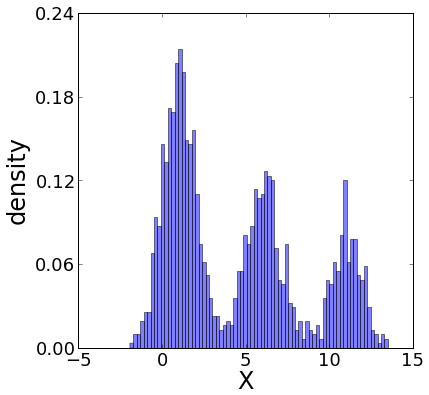
\includegraphics[width=0.7\textwidth, height=0.9\textheight, keepaspectratio]{_fig_01.png}
\par
\end{center}
\end{codeoutput}
\end{codecell}
Estimating a level set tree involves four main steps: estimating the
probability density function, constructing a similarity graph, finding
connected components over successively smaller subgraphs, and pruning
the tree. The geomTree method does all of these steps, and for most
applications is the easiest way to use DeBaCl. We can see what's in a
level set tree with the print function, although it's much easier to use
level set trees with the dendrogram visualization, available through the
plot method. Note that the plot method returns a tuple with several
objects; only the first is useful unless you want to modify the figure.

\begin{codecell}
\begin{codeinput}
\begin{lstlisting}
## Estimate the level set tree - the easy way
p_k = 0.02
k = int(p_k * n)
p_gamma = 0.05
gamma = int(p_gamma * n)

tree = gtree.geomTree(X, k, gamma, n_grid=None, verbose=True)
print tree

fig = tree.plot(form='lambda', width='uniform')[0]
fig.show()
\end{lstlisting}
\end{codeinput}
\begin{codeoutput}

\begin{verbatim}
iteration 0
iteration 100
iteration 200
iteration 300
iteration 400
iteration 500
iteration 600
iteration 700
iteration 800
iteration 900
iteration 1000
iteration 1100
iteration 1200
iteration 1300
iteration 1400
       alpha1    alpha2  children   lambda1   lambda2 parent  size
key                                                               
0    0.000000  0.018000    [1, 2]  0.000000  0.015621   None  1500
1    0.018000  0.041333    [3, 4]  0.015621  0.020742      0  1197
2    0.018000  0.699333        []  0.015621  0.150048      0   276
3    0.041333  0.627333  [27, 28]  0.020742  0.134807      1   731
4    0.041333  0.827333        []  0.020742  0.177435      1   439
27   0.627333  0.750667  [31, 32]  0.134807  0.161119      3   399
28   0.627333  0.863333        []  0.134807  0.187444      3    88
31   0.750667  0.916667        []  0.161119  0.208673     27    77
32   0.750667  1.000000        []  0.161119  0.294931     27   204

\end{verbatim}
\begin{center}
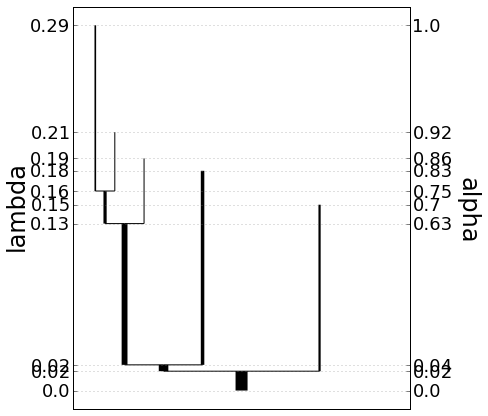
\includegraphics[width=0.7\textwidth, height=0.9\textheight, keepaspectratio]{_fig_03.png}
\par
\end{center}
\end{codeoutput}
\end{codecell}
While the level set tree plot offers a great deal of information about
the structure of the dataset, often the task is to assign a single
cluster label to each observation. DeBaCl offers several ways to
retrieve labels from a level set tree, through the getClusterLabels
function. Our preference is the `all-mode' method, which designates each
tree leaf as a cluster. The first-k option is appropriate if a specific
number of clusters is desired or known in advance, and the upper-set
option allows us to find clusters in a fraction of the data with highest
density.

\begin{codecell}
\begin{codeinput}
\begin{lstlisting}
## Retrieve cluster assignments from the tree
uc, leaves = tree.getClusterLabels(method='all-mode')
print "cluster counts:", np.bincount(uc[:, 1])
print "leaf indices:", leaves
\end{lstlisting}
\end{codeinput}
\begin{codeoutput}

\begin{verbatim}
cluster counts: [276 439  88  77 204]
leaf indices: [2, 4, 28, 31, 32]

\end{verbatim}

\end{codeoutput}
\end{codecell}
Generally speaking, retrieving clusters from a level set tree does not
assign every point to a cluster. In particular, once high-density
``foreground'' clusters are obtained, observations with low density must
be assigned to a group. This can be done with any classification method,
and DeBaCl includes a handful of options, including a k-nearest
neighbors classifier.

\begin{codecell}
\begin{codeinput}
\begin{lstlisting}
## Assign background points
fc = utl.assignBackgroundPoints(X.reshape((n, -1)), uc, method='knn', k=9)
print "final cluster counts:", np.bincount(fc[:, 1])
\end{lstlisting}
\end{codeinput}
\begin{codeoutput}

\begin{verbatim}
final cluster counts: [294 475 203 282 246]

\end{verbatim}

\end{codeoutput}
\end{codecell}
The four main phases of level set tree estimation can be done
individually for greater control of the methods and parameters. In this
example we use a kernel density estimator instead of the default
k-nearest neighbor estimator. For the sake of variety, the data are now
in $\mathbb{R}^2$, and the smoothness and pruning parameters are tweaked
to produce a reasonable tree. The scipy.stats package is loaded for the
kernel density estimate.

\begin{codecell}
\begin{codeinput}
\begin{lstlisting}
## Add the stats package for kernel density estimation
import scipy.stats as spstat

## Re-set data parameters
n = 1500
ctr = ((1, 5), (4, 5), (5, 1))
sdev = (0.5*np.eye(2),) * 3
mix = (0.5, 0.3, 0.2)


## Generate data
membership = np.random.multinomial(n, pvals=mix)
p = len(ctr[0])
X = np.zeros((n, p), dtype=np.float)
g = np.zeros((n, ), dtype=np.int)
b = np.cumsum((0,) + tuple(membership))

for i, (size, mu, sigma) in enumerate(zip(membership, ctr, sdev)):
	ix = range(b[i], b[i+1])
	X[ix, :] = np.random.multivariate_normal(mu, sigma, size)
	g[ix] = i


## Scatterplot, to show the simulation worked
fig, ax = plt.subplots()
ax.scatter(X[:,0], X[:,1], s=50, c=g, alpha=0.3)
fig.show()
\end{lstlisting}
\end{codeinput}
\begin{codeoutput}
\begin{center}
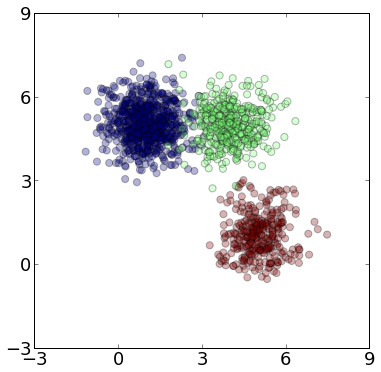
\includegraphics[width=0.7\textwidth, height=0.9\textheight, keepaspectratio]{_fig_06.png}
\par
\end{center}
\end{codeoutput}
\end{codecell}
The utils package (shortened to `utl' here for brevity) contains
functions to construct $k$-nearest neighbor and $\epsilon$-neighborhood
similarity graphs, although any similarity graph will work. Once the
similarity graph and density estimate are computed, the
constructDensityGrid method defines the relevant density levels and
finds the graph vertices removed from the similarity graph at each level
(called bg\_sets here). The program can be accelerated by using a grid
of density levels; here we use 300. The mode argument of this function
specifies if the grid should be built on density level values or blocks
of data points of equal size. The latter is specified by the `mass'
option. Finally, the constructTree method builds the level set tree.
Because our ordering function here is a density, we set the mode
argument to density. If the ordering function does not have a natural
floor of 0 (like a density or pseudo-density function), we set mode to
`general'.

\begin{codecell}
\begin{codeinput}
\begin{lstlisting}
## Construct the similarity graph and density estimate
p_k = 0.005
k = int(p_k * n)

W, k_radius = utl.knnGraph(X, k, self_edge=False)
kernel = spstat.gaussian_kde(X.T)
fhat = kernel(X.T)


## Construct the level set tree
bg_sets, levels = utl.constructDensityGrid(fhat, mode='mass', n_grid=300)
tree = gtree.constructTree(W, levels, bg_sets, mode='density', verbose=True)
print tree
\end{lstlisting}
\end{codeinput}
\begin{codeoutput}

\begin{verbatim}
iteration 0
iteration 100
iteration 200
       alpha1    alpha2 children   lambda1   lambda2 parent  size
key                                                              
0    0.000000  0.013333   [1, 2]  0.000000  0.004890   None  1500
1    0.013333  0.173333   [3, 4]  0.004890  0.022043      0  1167
2    0.013333  0.528000       []  0.004890  0.044852      0   313
3    0.173333  0.183333   [5, 6]  0.022043  0.022945      1  1040
4    0.173333  0.196667       []  0.022043  0.023848      1     1
5    0.183333  0.347333   [7, 8]  0.022945  0.034565      3  1028
6    0.183333  0.217333       []  0.022945  0.025501      3     2
7    0.347333  0.919333  [9, 10]  0.034565  0.097013      5   630
8    0.347333  0.698667       []  0.034565  0.059618      5   241
9    0.919333  1.000000       []  0.097013  0.109606      7   119
10   0.919333  0.936000       []  0.097013  0.099801      7     2

\end{verbatim}

\end{codeoutput}
\end{codecell}
Trees can be saved and loaded as MATLAB objects. This is shown here for
demonstration purposes, but is not necessary for this small dataset.
Pruning on the other hand, is necessary given that nodes with 1 or 2
members are likely due to random noise and should be removed.

\begin{codecell}
\begin{codeinput}
\begin{lstlisting}
## Save and/or load a tree (obviously redundant in this tutorial)
tree.save('test_tree')
tree = gtree.loadTree('test_tree')


## Prune the tree
p_gamma = 0.01
gamma = int(p_gamma * n)
tree.mergeBySize(gamma)
print tree
\end{lstlisting}
\end{codeinput}
\begin{codeoutput}

\begin{verbatim}
       alpha1    alpha2 children   lambda1   lambda2 parent  size
key                                                              
0    0.000000  0.013333   [1, 2]  0.000000  0.004890   None  1500
1    0.013333  0.347333   [7, 8]  0.004890  0.034565      0  1167
2    0.013333  0.528000       []  0.004890  0.044852      0   313
8    0.347333  0.698667       []  0.034565  0.059618      1   241
7    0.347333  1.000000       []  0.034565  0.109606      1   630

\end{verbatim}

\end{codeoutput}
\end{codecell}
The level set tree plot can act as very useful scaffold for exploring
spatially coherent subsets of data and the progression of high-density
clusters. The commands don't work well in an Ipython Notebook, but can
be uncommented and used at a regular Python or IPython command line.

\begin{codecell}
\begin{codeinput}
\begin{lstlisting}
## Interactive tools
#tool = gtree.ComponentGUI(tree, X, form='alpha', width='mass', output=['scatter'])
#tool = gtree.ClusterGUI(tree, X, form='alpha', width='mass', output=['scatter'])
#tool.show()
\end{lstlisting}
\end{codeinput}

\end{codecell}
Again we retrieve foreground cluter labels, although for this example we
suppose we know there are three clusters and use the first-K method. The
DeBaCl utils library includes the function plotForeground, for
visualizing foreground clusters in a 1-, 2- or 3-dimensional feature
space.

\begin{codecell}
\begin{codeinput}
\begin{lstlisting}
## Get foreground clusters and plot them
uc, nodes = tree.getClusterLabels(method='first-k', k=3)

fig, ax = utl.plotForeground(X, uc, s=50, alpha=0.5)
fig.show()
\end{lstlisting}
\end{codeinput}
\begin{codeoutput}
\begin{center}
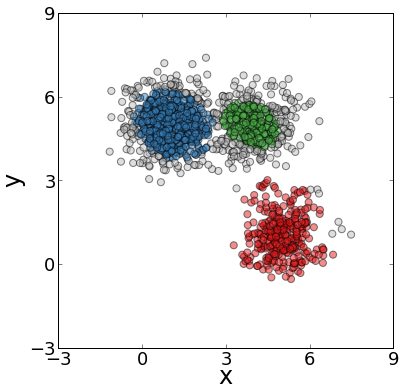
\includegraphics[width=0.7\textwidth, height=0.9\textheight, keepaspectratio]{_fig_09.png}
\par
\end{center}
\end{codeoutput}
\end{codecell}
Finally, the level set tree is plotted. The most basic form uses the
density scale (i.e. $\lambda$) as the dominant vertical axis, and spaces
the branches according to their mass (i.e.~fraction of data contained in
the maximal cluster of the branch). The nodes are colored to match the
foreground clusters above.

\begin{codecell}
\begin{codeinput}
\begin{lstlisting}
## Plot the basic level set tree with mass-based spacing
fig = tree.plot(form='lambda', width='mass', color_nodes=nodes)[0]
fig.show()
\end{lstlisting}
\end{codeinput}
\begin{codeoutput}
\begin{center}
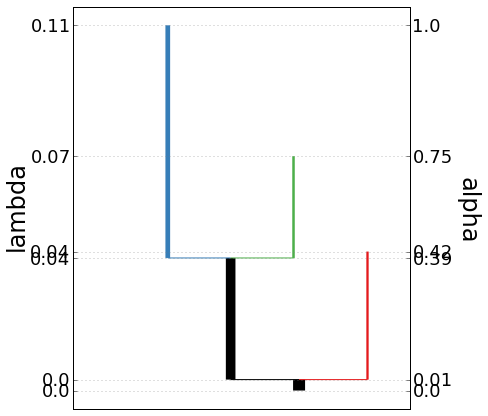
\includegraphics[width=0.7\textwidth, height=0.9\textheight, keepaspectratio]{_fig_10.png}
\par
\end{center}
\end{codeoutput}
\end{codecell}
The $\alpha$ scale shows the fraction of data excluded from the upper
level set for each value of $\lambda$. To use this more interpretable
scale, we change the form argument to `alpha'.

\begin{codecell}
\begin{codeinput}
\begin{lstlisting}
## Plot the level set tree with alpha scale
fig = tree.plot(form='alpha', width='mass', color_nodes=nodes)[0]
fig.show()
\end{lstlisting}
\end{codeinput}
\begin{codeoutput}
\begin{center}
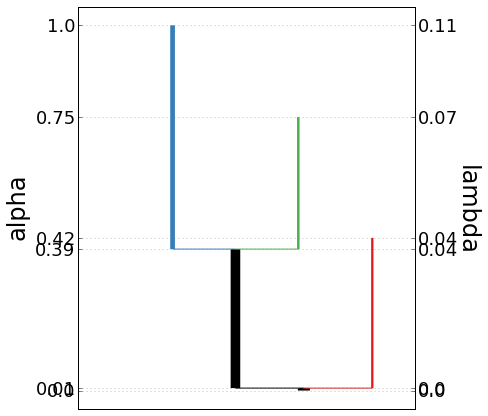
\includegraphics[width=0.7\textwidth, height=0.9\textheight, keepaspectratio]{_fig_11.png}
\par
\end{center}
\end{codeoutput}
\end{codecell}
The $\alpha$ scale improves interpetability in several ways. Because it
is based on mass, it is tempting to intuit that long vertical branches
in an $\alpha$ tree plot contain a lot of mass, but this intuition is
incorrect. To facilitate reading a plot this way, we use the $\kappa$
form of the tree, where each branch's height is proportional to its
salient mass. For leaf nodes, the salient mass is the fraction of points
in the cluster, and for internal nodes the salient mass is the mass of
the boundary region. In this example it does not look very different
from the $\alpha$ and $\lambda$ trees.

\begin{codecell}
\begin{codeinput}
\begin{lstlisting}
## Plot the level set tree with kappa scale
fig = tree.plot(form='kappa', width='mass', color_nodes=nodes)[0]
fig.show()
\end{lstlisting}
\end{codeinput}
\begin{codeoutput}
\begin{center}
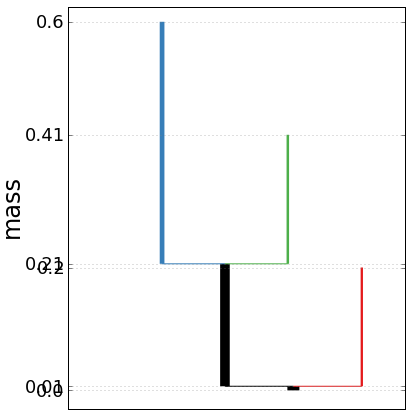
\includegraphics[width=0.7\textwidth, height=0.9\textheight, keepaspectratio]{_fig_12.png}
\par
\end{center}
\end{codeoutput}
\end{codecell}



\end{document}

